%% Paper on Elsevier's CAS template, two-column layout (cas-dc), target 12-15 pages.
%% Tables in tables/ and figures in figures/ are generated by scripts/build_paper.py; sections/ are written by
%% hand. Detailed material (per-instance tables, extra checks, further algorithms) is in supplement.tex.
%% Compile with pdflatex + bibtex (e.g. on Overleaf).

\documentclass[a4paper,fleqn]{cas-dc}

% If the frontmatter runs over more than one page use the longmktitle option.
%\documentclass[a4paper,fleqn,longmktitle]{cas-dc}

\usepackage[authoryear,longnamesfirst]{natbib}
\usepackage{rotating,algorithm,algpseudocode}

\newcommand{\ours}{DR-IMOEA}   % working name; rename here and in supplement.tex
\newcommand{\todo}[1]{\textbf{[TODO: #1]}}
\newcommand{\suppref}[1]{#1 of the supplementary material}

\begin{document}
\let\WriteBookmarks\relax
\def\floatpagepagefraction{1}
\def\textpagefraction{.001}

\shorttitle{Interval multi-objective DAG offloading in cloud--edge--end environments}
\shortauthors{TODO authors}

\title [mode = title]{Interval multi-objective offloading of DAG workflows in uncertain cloud--edge--end
  environments via decomposition-ranked three-tier environmental selection}

% TODO authors: copy the block below once per author and fill it in.
% Frontmatter macros process their arguments, so placeholders here are plain text (no \todo).
\author[1]{TODO First Author}[orcid=0000-0000-0000-0000]
\cormark[1]
\ead{todo@example.com}
\credit{TODO CRediT roles}
\affiliation[1]{organization={TODO organisation},
            city={TODO city},
            country={TODO country}}
\cortext[1]{Corresponding author}

% The CAS abstract environment writes its body to a side file, so the text must be inline here.
\begin{abstract}
Offloading tasks to edge servers or the cloud trades completion time against device energy and cost, under uncertain
bandwidth and server capacity. We formulate the offloading of directed acyclic graph (DAG) workflows over mobile devices,
edge servers and a cloud as an interval multi-objective problem: task placement and task order are optimised for
makespan along the interval critical path, device energy and cost, with uncertain quantities given as intervals.
Extending a recent reinforcement-learning-driven interval evolutionary algorithm to this problem, we show that its
convergence ranking, an interval dominance degree, stops selecting once most of the population is mutually
non-dominated, and that its learned control of the selection weights does not beat a fixed choice because the
per-generation reward is almost pure noise. The proposed \ours{} uses an interval best-position Tchebycheff rank as the
convergence tier of the dominance-, diversity- and uncertainty-aware three-tier selection, mates neighbours in
objective space and uses DAG-valid crossover and mutation. On 57 instances with up to 1000 tasks, it is compared with
four interval evolutionary algorithms, NSGA-II, NSGA-III, the reinforcement-learning-driven predecessor and
list-scheduling heuristics. \ours{} has the best IGD and hypervolume on all 12 instances of the predecessor's sizes and
beats the strongest baseline on 43 of 45 workflow instances in IGD and 42 in hypervolume, at a similar running time.
At 1000 and 2000 tasks it keeps the higher hypervolume, while IGD is level. A Monte Carlo check confirms that the
predicted objective intervals contain the realised values.
\end{abstract}

\begin{highlights}
\item Interval critical-path model for DAG workflow offloading in cloud--edge--end systems
\item Interval dominance degree loses selection pressure; a Tchebycheff rank restores it
\item Best IGD and hypervolume on all 12 instances of the predecessor's sizes
\item Beats IMOEA/D on 43 of 45 workflow instances in IGD at a similar running time
\item Learned DQN control of the selection weights does not beat a fixed choice
\end{highlights}

\begin{keywords}
Interval multi-objective optimisation \sep Computation offloading \sep DAG workflows \sep Cloud--edge--end computing
\sep Evolutionary algorithms \sep Uncertainty
\end{keywords}

\maketitle

% ---------------------------------------------------------------- body (rewritten section by section)
% Introduction (draft). Numbers from paper/tables (scripts/build_paper.py) and results/stats/a3_stall.csv.
\section{Introduction}
\label{sec:intro}

Mobile and Internet-of-Things devices run applications whose computation exceeds what the device can deliver within
its time and energy budget. Offloading parts of an application to edge servers close to the device, or further to a
cloud data centre, shortens execution but costs transmission time, energy and money, so where each part runs is a
multi-objective decision. Two features of real deployments make it hard. First, applications are rarely a single
task: a video analytics pipeline, a scientific workflow or a multi-stage inference service is a directed acyclic graph
(DAG) of tasks that exchange data, and the completion time is set by the longest chain of dependent computation and
transfer, not by any single task. Second, the quantities the decision depends on are uncertain at planning time:
wireless bandwidth fluctuates, servers are shared, and task workloads vary with their input. When only bounds on
these quantities are known, each objective becomes an interval, and the decision problem an interval multi-objective
optimisation problem.

Interval multi-objective evolutionary algorithms handle such problems by comparing solutions through interval
dominance and by rewarding solutions whose objective intervals are narrow \citep{limbourg2005ipmoea,jin2023imoeadawn,cui2024imeaied}.
The most recent of them for offloading, IMOEA-DQN \citep{jin2026imoeadqn}, selects each new population in three tiers:
a share $\alpha$ of the places by convergence (an interval dominance degree), a share $\beta$ by diversity (an interval
crowding distance) and a share $\gamma$ by uncertainty, and lets a deep Q-network choose $(\alpha, \beta, \gamma)$ in every
generation. It was formulated for independent tasks in a cloud--edge--end system with interval resources.

This paper extends that line of work to DAG applications and, in doing so, finds that two of its parts do not
carry over. The interval dominance degree loses its selection pressure: once most of the merged population is mutually
non-dominated, more pool members share the best value than there are convergence places, and the tier is filled by the
tie-break, at random. On our instances this happens for 86--100\% of the convergence places from generation 100 on, and
at the end of a run 117--121 of the 210 pool members share the best value for 88 places. On the 1000-task workflows the
backbone of IMOEA-DQN, run with the same fixed action as our method, ends with an IGD about six times higher. And the
learned controller of $(\alpha, \beta, \gamma)$ does not beat a well-chosen fixed action, because the per-generation reward it
learns from is almost pure noise.

We propose \ours{}, an interval multi-objective evolutionary algorithm for offloading DAG workflows in uncertain
cloud--edge--end environments. Its contributions are:
\begin{enumerate}
\item An interval critical-path model of DAG offloading over devices, edge servers and the cloud, with makespan, device
  energy and cost as interval objectives, task placement and task order as decision variables, and data transfer along
  every dependency. For single-task applications it reduces exactly to the model of \citet{jin2026imoeadqn}
  (Section~\ref{sec:model}).
\item A DAG-valid two-string encoding with precedence-preserving crossover and mutation, so that every offspring is
  feasible without repair (Section~\ref{sec:variation}).
\item A diagnosis of why the interval dominance degree stalls as a convergence tier, and a fix: an interval version of
  the best-position Tchebycheff rank of MSOPS \citep{hughes2003msops}, with ties broken by crowding distance, used as the
  convergence tier inside the three-tier selection, together with mating among neighbours in objective space
  (Sections~\ref{sec:stall} and~\ref{sec:rankc}). The rank itself is not new; its use inside the dominance-, diversity-
  and uncertainty-aware selection, the diagnosis and the evidence are.
\item An analysis of learned control of the selection weights: three learner designs with and without a
  graph-attention encoder of the DAG, and a reward audit that explains why none of them beats a fixed action
  (Section~\ref{sec:learned}).
\item An evaluation on 57 instances (Jin et al.'s instance sizes and five scientific workflow families with up to 1000
  tasks), plus 15 instances with 2000 tasks for scalability, against four interval evolutionary algorithms, NSGA-II,
  NSGA-III, IMOEA-DQN and list-scheduling heuristics, with a robustness check of the normalisation, a Monte Carlo check
  of the interval objectives against realised values, and an account of where the method is weaker
  (Sections~\ref{sec:experiments} and~\ref{sec:discussion}).
\end{enumerate}

On Jin et al.'s instance sizes \ours{} has the best IGD and hypervolume on all 12 instances, with 62\% lower mean IGD
than IMOEA/D. On the 45 workflow instances it is better than IMOEA/D on 43 instances in IGD and on 42 in hypervolume,
at about the same running time. At 1000 and 2000 tasks it keeps the hypervolume lead, while IMOEA/D covers the cheapest
schedules better and IGD is level.

Section~\ref{sec:related} reviews related work, Section~\ref{sec:model} states the model and
Section~\ref{sec:method} the method. Section~\ref{sec:experiments} reports the experiments,
Section~\ref{sec:discussion} discusses limitations, and Section~\ref{sec:conclusion} concludes.
          % 1   ~1.25 pages
% Related work (draft). Sources: docs/novelty_check.md (W1). \todo{} marks citations still to be found;
% refs marked VERIFY in refs.bib were read from abstracts only.
\section{Related work}
\label{sec:related}

\subsection{Offloading dependent tasks}
Offloading in mobile edge computing was first studied for independent tasks, where each task is placed on its own and
the objectives add up over tasks. Applications with dependent tasks need a scheduling view: the makespan follows the
critical path of the task graph, and the data passed between tasks cost time and energy whenever the two tasks run on
different nodes. List-scheduling heuristics such as HEFT \citep{topcuoglu2002heft} build a schedule task by task in a
priority order, and many multi-objective evolutionary algorithms optimise placement and order for crisp DAG
offloading in edge or cloud--edge--end systems \todo{cite 2--3 crisp DAG-offloading MOEAs}.
% Candidates in docs/novelty_check.md: the FGCS 2023 MOEA/D cloud-edge-end paper, the FGCS 2025 IIoT dependency-aware paper.
These models treat bandwidth, CPU speed and workload as known values.
% VERIFY against the full text of Shi et al. (only the abstract was read): migration rather than placement, no cloud tier.
\citet{shi2023workflowmigration} consider
dependent workflows with interval bandwidth and computing power, but for workflow migration between edge servers
rather than placement and ordering over devices, edge servers and the cloud. Our model is the first, to our knowledge,
to compute interval makespan along the critical path of a DAG over all three tiers, with both placement and order as
decision variables, and it reduces to the independent-task model of \citet{jin2026imoeadqn} when every
application has one task.

\subsection{Interval multi-objective evolutionary algorithms}
Interval multi-objective problems are solved either by turning them into crisp problems, for example through interval
midpoints and widths, or by comparing intervals directly. IP-MOEA \citep{limbourg2005ipmoea} extends Pareto dominance to
interval vectors and crowds by hypervolume contributions of the interval bounds. Decomposition-based methods compare
solutions on scalarised subproblems: IMOEA/D-AWN \citep{jin2023imoeadawn} adapts the weight vectors and neighbourhood sizes
using an interval sparsity measure, and IMOEA/D-DAW \citep{zhang2026imoeaddaw} uses interval Tchebycheff and penalty-based
scalarisations with dynamic neighbourhoods for robot path planning. IMEA-IED \citep{cui2024imeaied} compares intervals by
an information-entropy dominance and selects within niches. IMaOEACI \citep{cai2025imaoeaci} steers an interval
many-objective search by an individual comprehensive indicator for vehicle selection in federated learning. IMOEA-DQN \citep{jin2026imoeadqn} is the method closest to ours: a three-tier
environmental selection by interval dominance degree, interval crowding distance and uncertainty dominance, with the
shares chosen by a deep Q-network \citep{mnih2015dqn}. None of these methods uses a weight-vector rank as one tier of a
dominance-, diversity- and uncertainty-aware selection.

\subsection{Combining dominance and decomposition}
The loss of selection pressure when most of a population is non-dominated is well known for problems with many
objectives \citep{ishibuchi2008review}; we show that it already occurs with three interval objectives under
possibility-degree dominance. Several crisp algorithms combine Pareto dominance with weight vectors or reference
points: NSGA-III \citep{deb2014nsga3} niches the last front by reference directions, MOEA/DD \citep{li2015moeadd} uses
dominance and decomposition together, and $\theta$-DEA \citep{yuan2016thetadea} defines a dominance relation on
decomposition distances. The rank \ours{} uses comes from MSOPS \citep{hughes2003msops}, which ranks a solution by its best
position over the orderings induced by a set of weighted min--max scores; Global WASF-GA \citep{saborido2017gwasfga}
classifies a population into fronts by achievement scalarising functions over weight vectors. \ours{} applies the
MSOPS rank to interval midpoints and uses it as the convergence tier inside the three-tier selection, which keeps the
diversity and uncertainty tiers of the interval setting.

\subsection{Learned control of evolutionary algorithms}
Reinforcement learning has been used to choose operators, parameters or selection weights of evolutionary algorithms
online \todo{cite a survey of RL-assisted EAs}. IMOEA-DQN \citep{jin2026imoeadqn} learns the selection
weights from the change in a population indicator after every generation. Negative results are rarely reported; our
analysis in Section~\ref{sec:learned} shows that for this problem the per-generation reward is too noisy, and the room
for an adaptive schedule too small, for learned control to beat a fixed action, and that a graph-attention
encoder \citep{velickovic2018gat} of the DAG does not change this.
        % 2   ~1 page
% Problem formulation (condensed for the two-column paper, step 2). Matches gat_imoea_dqn/evaluator.py,
% intervals.py and dataset_tools/loader.py with EvaluatorConfig(energy_scope="device", external_io="device",
% makespan="sum_apps").
\section{Problem formulation}
\label{sec:model}

\subsection{Interval numbers}
\label{sec:intervals}
An uncertain quantity is an interval $\tilde a = [a^L, a^U]$ with midpoint $m(\tilde a)$ and width $w(\tilde a) =
a^U - a^L$. Every operation of the model (sum, maximum, and a positive quantity divided by a positive interval) is
monotone in each bound, so it is applied to the lower and to the upper inputs, e.g.\ $\tilde C / \tilde f = [C^L / f^U,
C^U / f^L]$. Intervals are compared by the possibility degree \citep{jin2026imoeadqn}
\begin{equation}
P(\tilde a \le \tilde b) = \min\Big\{1, \max\Big\{0, \frac{b^U - a^L}{w(\tilde a) + w(\tilde b)}\Big\}\Big\}.
\label{eq:possibility}
\end{equation}
Solution $x$ \emph{interval-dominates} $y$ ($x \prec_{IN} y$) when $P(\tilde F_m(x) \le \tilde F_m(y)) \ge 0.5$ for every
objective $m$, with strict inequality for at least one. The uncertainty of a solution is measured by $U_1 = \sum_m
w(\tilde F_m)$ and $U_2 = \prod_m w(\tilde F_m)$ on normalised objectives.

\subsection{System and application model}
The system (Fig.~\ref{fig:system_model}) follows \citet{jin2026imoeadqn}: $D$ mobile devices, $n$ edge servers and a
cloud. Device $d$ has CPU frequency $\tilde f_d$, energy per cycle $\tilde e_d$, transmit power $p_d$ and idle power
$p^{idle}_d$, and reaches the edge servers within its range at the wireless rate $\tilde R_{d,u} = \tilde B \log_2(1 + p_d
g / v_0)$. Edge server $u$ shares its frequency $\tilde f_u$ equally among the tasks placed on it, and the cloud gives
every task $\tilde f_C$. Edge servers are linked to each other and to the cloud at rates $\tilde W_E$ and $\tilde W_C$; a
device reaches the cloud through its nearest edge server.

Each device submits one application, a DAG of tasks; together they form $\mathcal{G} = (V, E)$ with $K = |V|$. Task $k$
has workload $\tilde C_k$ cycles, arc $(p, k)$ carries $\tilde D_{pk}$ bits, and a task may read input from and return
output to its device. A task starts only after all its predecessors have finished and their data have arrived. With one
task per application the model reduces to that of \citet{jin2026imoeadqn}.

A solution is a pair $(\mathbf{x}, \mathbf{o})$. The allocation string $\mathbf{x} \in \{0, \dots, n+1\}^K$ places each
task on its device ($0$), an edge server ($1..n$) or the cloud ($n+1$); the priority string $\mathbf{o}$ is a topological
order of $\mathcal{G}$ that fixes the dispatch order.

\subsection{Interval critical-path timing}
Task $k$ runs at $\tilde f_k = \tilde f_d$, $\tilde f_u / n_u$ or $\tilde f_C$ for $n_u$ tasks on server $u$, so it
computes for $\tilde t_k = \tilde C_k / \tilde f_k$. Visiting the tasks in the order $\mathbf{o}$,
\begin{align}
\widetilde{AT}_k &= \max\Big\{\tilde\tau^{in}_k, \max_{(p, k) \in E} \Big(\widetilde{FT}_p + \frac{\tilde D_{pk}}{\tilde R(x_p, x_k)}\Big)\Big\}, \label{eq:at}\\
\widetilde{FT}_k &= \max\{\widetilde{AT}_k, \widetilde{av}(x_k)\} + \tilde t_k, \label{eq:ft}
\end{align}
where $\tilde\tau^{in}_k$ is the upload time of $k$'s input if $k$ is offloaded, transfers between co-located tasks
take no time, and $\widetilde{av}(x_k)$ is the finish time of the previous task on the same device, since a device runs
one task at a time. Maxima are taken boundwise; the chain that sets the latest finish time is the \emph{interval
critical path}.

\subsection{Objectives and problem}
The objectives are the total makespan, the devices' energy and the monetary cost:
\begin{align}
\tilde F_1 &= \sum_{a} \max_{k \in V_a} \big(\widetilde{FT}_k + \tilde\tau^{out}_k\big), \label{eq:f1}\\
\tilde F_2 &= \sum_{x_k = 0} \tilde C_k \tilde e_{d(k)} \nonumber\\
  &\quad + \sum_{x_k \ne 0} \Big(p_{d(k)} \frac{\tilde D^{in}_k}{\tilde R_{d(k), x_k}} + p^{idle}_{d(k)} \tilde t_k\Big) \nonumber\\
  &\quad + \sum_{\substack{(p, k) \in E:\\ x_p = 0,\, x_k \ne 0}} p_{d(p)} \frac{\tilde D_{pk}}{\tilde R_{d(p), x_k}}, \label{eq:f2}\\
\tilde F_3 &= \eta_E \sum_{1 \le x_k \le n} \tilde f_k \tilde t_k + \eta_C \sum_{x_k = n+1} \tilde t_k, \label{eq:f3}
\end{align}
where $V_a$ are the tasks of application $a$, $\tilde\tau^{out}_k$ the time to return $k$'s output and $d(k)$ its
device. $\tilde F_2$ counts local computation, transmission to offloaded tasks (for the cloud, up to the nearest edge
server, idling while the data cross $\tilde W_C$) and idle waiting, i.e.\ the devices'
energy only, as in \citet{jin2026imoeadqn} (all-tier energy is a sensitivity case in Section~\ref{sec:sensitivity});
$\eta_E$ and $\eta_C$ are the edge and cloud prices. The problem is
\begin{equation}
\min_{(\mathbf{x}, \mathbf{o})} \big(\tilde F_1, \tilde F_2, \tilde F_3\big)\ \text{s.t.}\ x_k \in \mathcal{A}_k\, \forall k,\
\mathbf{o}\ \text{topol.},
\label{eq:problem}
\end{equation}
where $\mathcal{A}_k$ are the nodes reachable from $k$'s device; we seek the solutions that no other solution
interval-dominates. Scheduling a DAG on heterogeneous processors is NP-hard even with crisp data
\citep{topcuoglu2002heft}, which motivates an evolutionary approach.
          % 3   ~1.5 pages
% Method section (draft). Numbers: A1 / A1b ablation (paper/tables/ablation.tex), A2 action sweep
% (results/experiments/action_sweep/summary.md), A3 stall and trade-off (results/stats/a3_stall.csv,
% results/figures/a3_*). Settings: scripts/experiment.py POLICIES["final"].
\section{The proposed method: \ours{}}
\label{sec:method}

\ours{} keeps the evolutionary framework of IMOEA-DQN~\cite{jin2026imoeadqn} wherever the DAG model allows and changes
it in three places. First, the convergence ranking of the three-tier environmental selection, Jin et al.'s interval
dominance degree, is replaced by a decomposition rank that does not lose its selection pressure once most of the
population is mutually non-dominated (Sections~\ref{sec:stall}--\ref{sec:rankc}). Second, parents mate with
neighbours in objective space (Section~\ref{sec:variation}). Third, the selection weights $(\alpha, \beta, \gamma)$,
which IMOEA-DQN chooses every generation with a deep Q-network, are fixed to a value chosen on training instances
(Section~\ref{sec:weights}); Section~\ref{sec:learned} shows that the learned controller does not beat it.
Algorithm~\ref{alg:main} gives the main loop.

\subsection{Encoding and variation}
\label{sec:variation}
A solution is the pair $(\mathbf{x}, \mathbf{o})$ of Section~\ref{sec:model}. The initial population draws every
allocation gene uniformly from the nodes the task's device can reach and every priority string from a randomised
Kahn's algorithm, which picks uniformly among the ready tasks. Algorithm~\ref{alg:var} creates one child per member of
the population. The partner of member $i$ is drawn from its $T$ nearest neighbours by Euclidean distance between
normalised interval midpoints, the mating restriction of MOEA/D~\cite{zhang2007moead}. Crossover keeps the
dual-adaptive scheme of Jin et al.: the crossover probability is 0.7 for the better half of the population by
uncertainty front and 0.9 for the other half, and the allocation string is recombined gene by gene (DAEC), taking each
gene from either parent with equal probability. Jin et al.'s simulated binary crossover cannot be applied to a task
order, so the priority strings are recombined by precedence-preserving order-based crossover
(POX)~\cite{bierwirth1996permutation}: a random binary mask decides, position by position, which parent supplies its
leftmost task not yet used, and any mask yields a topological order. Mutation reassigns each allocation gene with
probability $1/K$ to another reachable node and moves each task with probability $1/K$ to a random position after its
last predecessor and before its first successor. Every child is therefore feasible by construction.

\subsection{Three-tier environmental selection}
Jin et al.'s selection ranks the merged population $P \cup Q$ of $2N$ solutions in three ways:
\begin{itemize}
\item \emph{Rank C} (convergence): the interval dominance degree $R_{IN}(x) = \sum_{y \prec_{IN} x} S(y)$, where $S(y)$ is
  the number of pool members $y$ interval-dominates; lower is better.
\item \emph{Rank D} (diversity): the interval crowding distance $\mathrm{ICD}(x) = \sum_{y} \mathrm{ICD}(x, y)$ over the
  $k = \mathrm{round}(\sqrt{2N})$ most similar solutions $y$, with
  $\mathrm{ICD}(x, y) = \sum_m |m(\tilde F_m(x)) - m(\tilde F_m(y))| / (\mu(x, y) + V(x) + V(y) + 1)$, where $V$ is the
  volume of a solution's objective box and $\mu$ the overlap volume of two boxes; higher is better.
\item \emph{Rank U} (uncertainty): the dominance degree $R_U$ under Pareto dominance on $(U_1, U_2)$; lower is better.
\end{itemize}
Given $(\alpha, \beta, \gamma)$ with $\alpha + \beta + \gamma = 1$, the next population takes the best $\mathrm{round}(\alpha N)$
solutions by Rank C, then the best $\mathrm{round}(\beta N)$ not yet chosen by Rank D, and the rest by Rank U
(Algorithm~\ref{alg:sel}). Exact copies of a chosen genotype are skipped, so clones cannot fill the population.

\subsection{Why the interval dominance degree stalls}
\label{sec:stall}
$R_{IN}$ separates solutions only while some of them dominate others. Under interval dominance two solutions are
incomparable whenever their intervals overlap enough in some objective, so after a few hundred generations most of the
merged population has $R_{IN} = 0$. When more than $\alpha N$ pool members share the best value, Rank C no longer
selects: the $\alpha N$ convergence places are filled by the tie-break, which Jin et al.\ leave unspecified and which
is random in a literal implementation. Figure~\ref{fig:a3_stall} measures this on two instances. With $R_{IN}$, the
share of Rank C places decided by the tie-break rises to 86--100\% after generation 100 and to almost 100\% after
generation 500, when 117--121 of the 210 pool members share $R_{IN} = 0$ for $\alpha N = 88$ places. The convergence tier
then draws at random from the first front, and the population drifts along it instead of approaching the Pareto front.
The effect grows with the size of the DAG: the fixed-action Jin backbone has a mean IGD of 0.052 on the 100-task
workflows of Suite~B and 0.175 on the 1000-task ones (Section~\ref{sec:results}).

\subsection{Tchebycheff Rank C}
\label{sec:rankc}
\ours{} replaces $R_{IN}$ by a rank that orders every solution. Let $W$ be a set of $N$ Das--Dennis weight vectors and let
$G^L, G^U$ be the objectives scaled per objective to $[0, 1]$ over the pool. For each $\mathbf{w} \in W$ the interval
Tchebycheff value of a solution is
\begin{equation}
\tilde g(x \mid \mathbf{w}) = \Big[\max_m w_m G^L_m(x), \; \max_m w_m G^U_m(x)\Big],
\label{eq:tch}
\end{equation}
and the pool is sorted by it. Sorting intervals by the possibility degree~\eqref{eq:possibility} at threshold 0.5 is
sorting by midpoint, which is how IMOEA/D compares two solutions on a subproblem. Let $\pi_{\mathbf{w}}(x) \in
\{0, \dots, 2N - 1\}$ be the position of $x$ when the pool is sorted by ascending $m(\tilde g(\cdot \mid \mathbf{w}))$.
The new Rank C of a solution is its best position over all these orders,
\begin{equation}
R_C(x) = \min_{\mathbf{w} \in W} \pi_{\mathbf{w}}(x),
\label{eq:rankc}
\end{equation}
so the best solution of every subproblem has $R_C = 0$, and a solution is ranked well when it is close to the best on at
least one direction. This is the ranking of MSOPS~\cite{hughes2003msops} applied to interval midpoints. What \ours{}
adds is its use as the convergence tier inside the dominance-, diversity- and uncertainty-aware selection of Jin et al.,
with ties broken by descending interval crowding distance rather than at random. With this rank the share of
convergence places decided by the tie-break stays at 11--23\% throughout the run (Fig.~\ref{fig:a3_stall}). Unlike
MOEA/D-style methods, \ours{} keeps a generational population and Jin et al.'s diversity and uncertainty tiers.

\subsection{Selection weights}
\label{sec:weights}
The weights $(\alpha, \beta, \gamma)$ are fixed to $(5/6, 1/6, 0)$, which gives 88 places by Rank C and 17 by Rank D in
a population of 105. The value was chosen before any test run by holding each of the 28 actions of IMOEA-DQN's action
set fixed on 36 training instances that are separate from the test instances (three further instances of each Suite~A
configuration, with data $\times 1$ and $\times 20$). It had the best mean IGD rank (2.25 of 28); on average its IGD was 1.13 times
the best action's on each instance, and 1.71 times at worst. Only four actions, all with $\alpha \ge 2/3$, were ever
best on an instance. The other weights trade convergence for precision along one curve
(Fig.~\ref{fig:a3_tradeoff}): a small uncertainty share, $(5/6, 0, 1/6)$, lowers the imprecision per solution by 10\%
for an IGD ratio of 1.15 instead of 1.13, while more weight on Rank D or Rank U raises IGD steeply. The neighbourhood
size $T = 10$ and the probability of mating with a neighbour, 1.0, were tuned on the same training instances.

% Computational complexity (R2). Derived from the code (gat_imoea_dqn/operators.py, selection.py,
% intervals.py, evaluator.py); measured times in Table~\ref{tab:timing} (scripts/build_paper.py).
\subsection{Computational complexity}
\label{sec:complexity}

Let $N$ be the population size, $M = 3$ the number of objectives, $K = |V|$ and $|E|$ the numbers of tasks
and data dependencies, and $F$ the number of interval non-dominated fronts in a population
($F \le N$, and small in practice because most of the population soon shares the first front).
One generation of \ours{} costs the following.

\begin{itemize}
\item \emph{Variation} (Algorithm~\ref{alg:var}). The interval dominance matrix of $P$ takes $O(MN^2)$ and peeling
  its fronts $O(FN^2)$; the uncertainty fronts on $(U_1, U_2)$ take the same. The neighbourhoods need all pairwise
  midpoint distances, $O(MN^2)$, and a sort of each row, $O(N^2 \log N)$. Building one child takes $O(K + |E|)$:
  DAEC and POX are linear in $K$, a shift mutation moves a task within its precedence window in $O(K)$, and with
  mutation rate $1/K$ one task moves per child in expectation. In total $O\big(N^2(M + F + \log N) + N(K + |E|)\big)$.
\item \emph{Evaluation} (Algorithm~\ref{alg:eval}). The interval critical-path calculus visits every task and every
  dependency once, $O(K + |E|)$ per solution and $O\big(N(K + |E|)\big)$ per generation.
\item \emph{Selection} (Algorithm~\ref{alg:sel}) on the pool of $2N$. The Tchebycheff values for $N$ weight vectors take
  $O(MN^2)$ and sorting the pool once per vector $O(N^2 \log N)$; the interval crowding distance needs all pairs,
  $O(MN^2)$; the uncertainty dominance degree $O(N^2)$; filling the three tiers with genotype de-duplication $O(NK)$.
  In total $O\big(N^2(M + \log N) + NK\big)$.
\end{itemize}

A generation therefore costs $O\big(N^2(M + F + \log N) + N(K + |E|)\big)$, and a run of $G_{\max}$ generations
$O\big(G_{\max}[N^2(M + F + \log N) + N(K + |E|)]\big)$ time with $O(N^2 + NK)$ memory. Jin et al.'s Rank C, the
interval dominance degree $R_{IN}$, costs $O(MN^2)$ for the dominance matrix plus $O(N^2)$ for the degrees, so the
Tchebycheff Rank C adds only the $O(N^2 \log N)$ of the per-vector sorts; neighbourhood mating adds the same order.
Neither changes the number of evaluations, which is $N(G_{\max} + 1)$ for \ours{} and every baseline.

With $N = 105$ the population terms are about $N^2(M + \log_2 2N) \approx 1.2 \times 10^5$ elementary operations per
generation, while the evaluation term $N(K + |E|)$ grows from about $3 \times 10^4$ for the 100-task Cybershake
workflow ($|E| = 192$) to $3 \times 10^5$ at 1000 tasks and $6 \times 10^5$ at 2000. The measured times
(Table~\ref{tab:timing}) show that \ours{} needs about as long as IMOEA/D and the fixed-action Jin backbone on every
instance, and that its time grows only 1.8-fold from 100 to 2000 Cybershake tasks: the evaluation loop is compiled and
has a small constant, so the population terms, which do not depend on $K$, account for most of the run time. The
learned controller of IMOEA-DQN adds a state computation and a network forward pass every generation and a training
step every 50 generations; on the same instances this costs 2--52\% more time than the fixed-action backbone, without
improving the result (see the analysis of learned control in the paper).

         % 4   ~2.5 pages
% Experiments (condensed for the two-column paper, step 4). Numbers from paper/tables/* (scripts/build_paper.py),
% results/stats/e5_convergence.*, results/stats/e7_montecarlo.*; supplement items cited with \Sref.
\section{Experiments}
\label{sec:experiments}

\subsection{Setup}
\label{sec:setup}
\emph{Suite A} reproduces the instance sizes of \citet{jin2026imoeadqn}: 3, 6 or 10 edge servers, 100, 300 or 500 tasks,
and 20--250 devices that each submit a layered random DAG. Workloads are 1--5 Gcycles and data 500--3000 KB as in Jin et
al., used as given and multiplied by 20; this gives 12 test instances. 36 further instances generated with other seeds
were used only to set the method's parameters. \emph{Suite B} takes five scientific workflow families from WfCommons
\citep{coleman2022wfcommons} (Cybershake, Epigenomics, Inspiral, Montage, Sipht) with 100, 400 and 1000 tasks in Jin et
al.'s small scenario (3 edge servers, 6 devices), with sizes mapped into Jin et al.'s ranges, interval half-widths of
5--30\% and data multiplied by 1, 20 or 100: 45 instances. Table~\Sref{tab:params} of the supplementary material lists all
parameters.

We compare \ours{} with four interval evolutionary algorithms, IMOEA/D with the original settings reported by
\citet{cui2024imeaied}, IMOEA/D-AWN \citep{jin2023imoeadawn}, IMEA-IED \citep{cui2024imeaied} and IP-MOEA
\citep{limbourg2005ipmoea}; with NSGA-II \citep{deb2002nsga2} on interval midpoints or by interval dominance and NSGA-III
\citep{deb2014nsga3}; and with IMOEA-DQN \citep{jin2026imoeadqn} and its backbone run with the fixed action
$(5/6, 1/6, 0)$ (the \emph{Jin backbone}), which isolates the effect of Rank C and the mating. All methods share the
encoding, operators, evaluator, $N = 105$ and the budget of $N(G_{\max}+1)$ evaluations with $G_{\max} = 1000$.
IGD is measured on interval midpoints against the non-dominated union of all final fronts, and HV is the mean of the
lower- and upper-bound hypervolumes (reference 1.1), both after normalising each instance once over all methods.
\ours{}, IMOEA/D and the Jin backbone were run 30 times, the others 10 times; methods are compared per instance by the
Wilcoxon rank-sum test with Holm's correction \citep{holm1979} and over instances by Friedman ranks \citep{demsar2006}.

% generated by scripts/build_paper.py; do not edit by hand
\begin{table*}[!htbp]
\centering
\footnotesize
\caption{Results on both suites: mean IGD ($\times10^{-2}$) and HV over instances, the number of instances on which each method is significantly better / worse / not different from \ours{} (Wilcoxon rank-sum, Holm-corrected, $\alpha = 0.05$), and the mean Friedman rank by IGD (Nemenyi critical difference 3.91 on Suite A, 2.02 on Suite B). Per-instance results are in the supplementary material.}
\label{tab:summary}
\setlength{\tabcolsep}{3pt}
\begin{tabular}{lcccccccccc}
\toprule
& \multicolumn{5}{c}{Suite A (12 instances)} & \multicolumn{5}{c}{Suite B (45 instances)} \\
\cmidrule(lr){2-6}\cmidrule(lr){7-11}
Method & IGD & HV & IGD $+/-/\approx$ & HV $+/-/\approx$ & Rank & IGD & HV & IGD $+/-/\approx$ & HV $+/-/\approx$ & Rank \\
\midrule
\ours{} & \textbf{1.22} & \textbf{0.819} & -- & -- & 1.00 & \textbf{1.86} & \textbf{0.949} & -- & -- & 1.29 \\
IMOEA/D & 3.19 & 0.797 & 0/12/0 & 0/12/0 & 2.83 & 2.57 & 0.935 & 1/43/1 & 2/42/1 & 2.69 \\
IMOEA/D-AWN & 2.91 & 0.797 & 0/12/0 & 0/12/0 & 2.42 & 4.44 & 0.915 & 0/43/2 & 0/44/1 & 3.29 \\
IMEA-IED & 12.40 & 0.691 & 0/12/0 & 0/12/0 & 7.17 & 13.34 & 0.828 & 0/45/0 & 0/45/0 & 7.73 \\
IP-MOEA & 14.71 & 0.658 & 0/12/0 & 0/12/0 & 8.50 & 12.24 & 0.822 & 0/45/0 & 0/45/0 & 6.98 \\
NSGA-II (mid) & 4.84 & 0.770 & 0/12/0 & 0/12/0 & 4.50 & 6.51 & 0.882 & 4/40/1 & 0/44/1 & 3.82 \\
NSGA-II (int) & 4.80 & 0.771 & 0/12/0 & 0/12/0 & 4.25 & 6.57 & 0.882 & 5/40/0 & 0/44/1 & 4.09 \\
NSGA-III & 13.61 & 0.690 & 0/12/0 & 0/12/0 & 7.75 & 15.42 & 0.822 & 0/45/0 & 0/45/0 & 8.40 \\
Jin backbone & 11.66 & 0.635 & 0/12/0 & 0/12/0 & 6.67 & 11.64 & 0.805 & 0/45/0 & 0/45/0 & 6.78 \\
IMOEA-DQN & 25.43 & 0.605 & 0/12/0 & 0/12/0 & 9.92 & 22.94 & 0.736 & 0/45/0 & 0/45/0 & 9.93 \\
\bottomrule
\end{tabular}
\end{table*}


\subsection{Comparison with the baselines}
\label{sec:results}
Table~\ref{tab:summary} summarises both suites. On Suite A, \ours{} has the best IGD and HV on all 12 instances, with a
mean IGD 62\% below IMOEA/D's and Friedman rank 1.00. On Suite B it is better than IMOEA/D on 43 of 45 instances in IGD
and 42 in HV; IMEA-IED, IP-MOEA, NSGA-III, the Jin backbone and IMOEA-DQN lose on every instance, and IMOEA/D-AWN is never
better. NSGA-II reaches a lower IGD on 4--5 instances, all 100-task workflows with data $\times 1$, and never a higher HV.
The Jin backbone, with the same fixed action, has a six times higher IGD (0.116), and its gap grows with the DAG, as
Section~\ref{sec:stall} predicts. The intervals of \ours{} are slightly wider than IMOEA/D's (Suite B imprecision 60.9
against 57.8; Table~\Sref{tab:suiteb_imprecision}); the methods with narrower intervals keep much smaller fronts.
Per-instance results are in Tables~\Sref{tab:suitea_igd}--\Sref{tab:suiteb_hv_jin} and list-scheduling heuristics,
16--33 times worse in IGD, in Table~\Sref{tab:heuristics}.

The comparison with IMOEA/D depends on the normalisation at one size only. Repeating it with four different method
pools defining the normalisation and the reference front (Table~\Sref{tab:robustness}) leaves every verdict on Suite A
and up to 400 tasks, and every HV verdict, unchanged; at 1000 tasks, however, IMOEA/D has the lower IGD on 6--9 of 15
instances when only the strong methods form the pool. We therefore read the 1000-task results on HV, where \ours{} is
better on 12 of 15.

\subsection{Convergence and ablation}
\label{sec:convergence}
\label{sec:ablation}
Fig.~\ref{fig:e5_convergence} shows that \ours{} pulls ahead of every method by generation 100 on medium-250 and ends
with a third of IMOEA/D's IGD (0.012 against 0.035). On montage-400, IMOEA/D converges faster at first and \ours{}
overtakes it at about generation 350. On the 1000-task workflows the two are close throughout, \ours{} ends slightly
ahead, and both curves are still falling at generation 1000. IMOEA-DQN starts worse than the initial population because
its early actions concentrate the search in one region.

\begin{figure*}[pos=tbp]
\centering
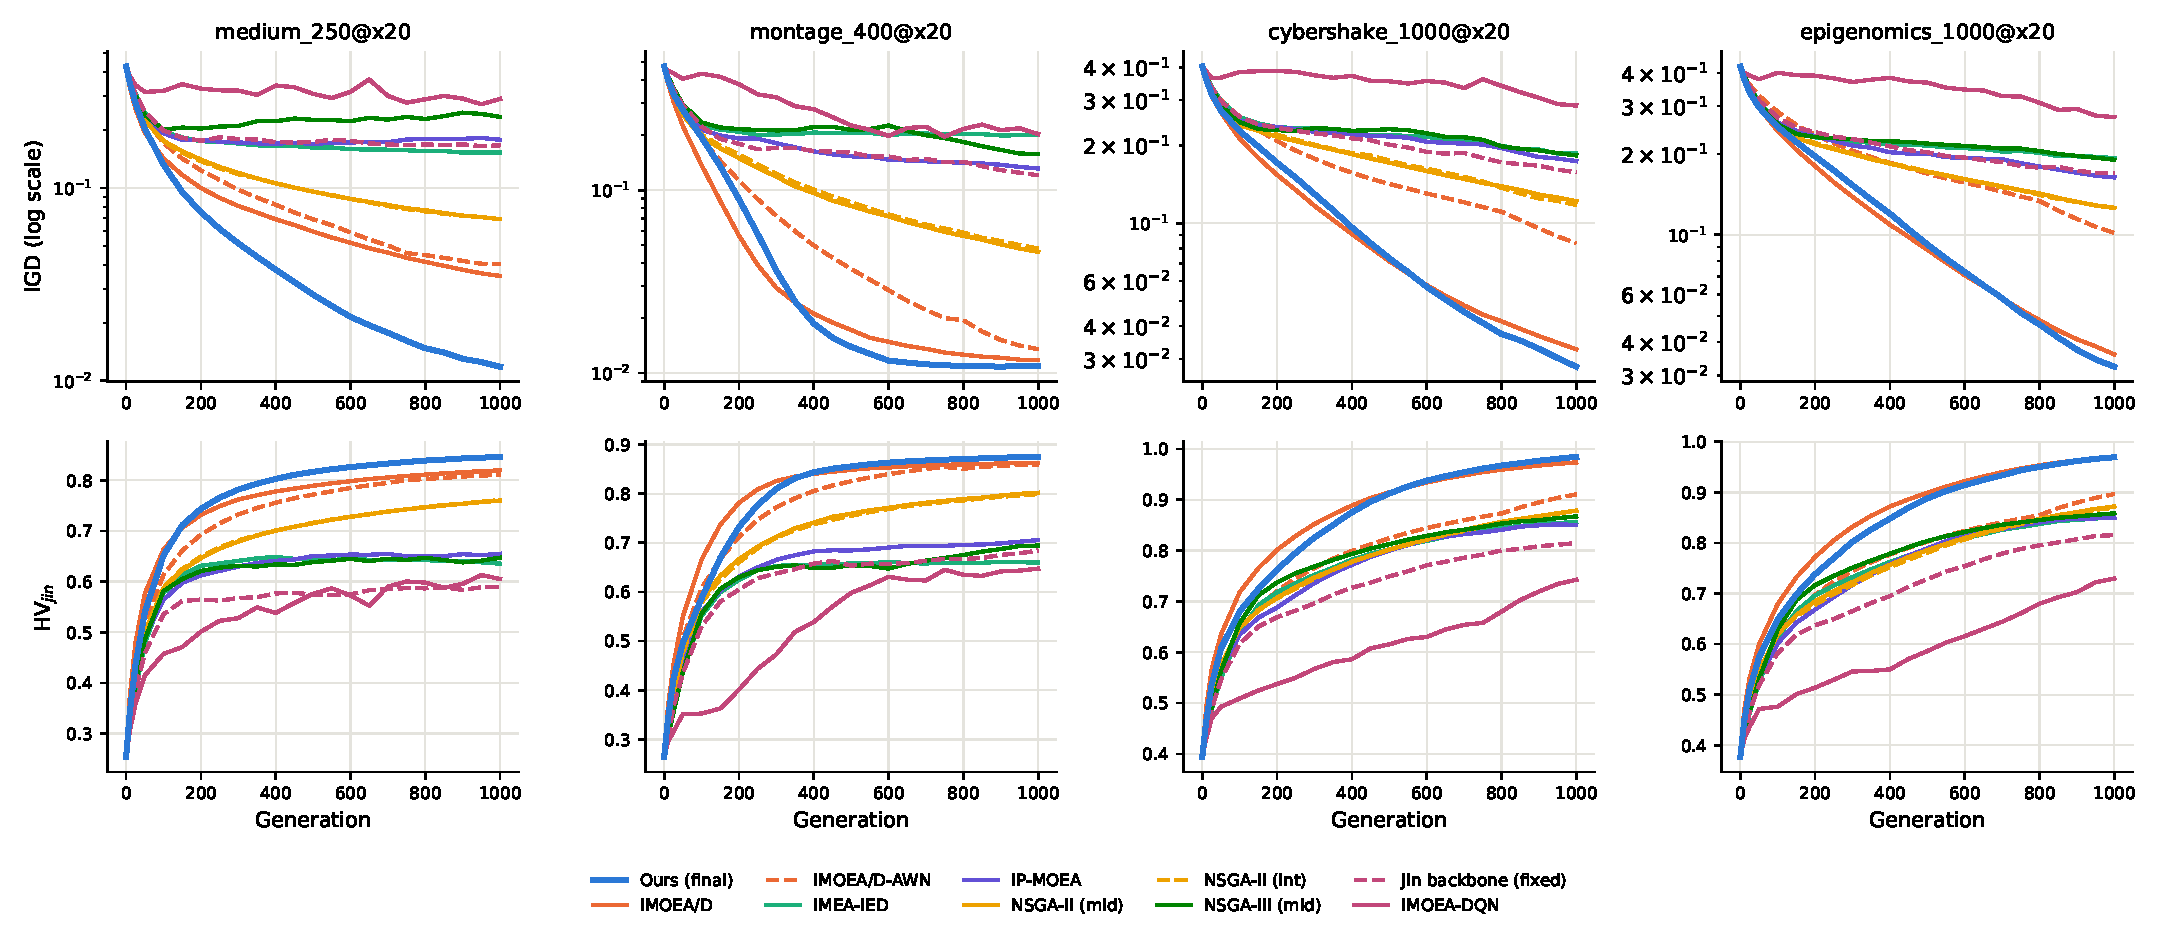
\includegraphics[width=\textwidth]{figures/e5_convergence.pdf}
\caption{Mean IGD (top, log scale) and HV (bottom) against the generation, 10 runs per method, on one Suite A and three
Suite B instances (data $\times 20$).}
\label{fig:e5_convergence}
\end{figure*}

Table~\ref{tab:ablation} builds \ours{} from the Jin backbone. The Tchebycheff Rank C halves the IGD, the ICD tie-break
lowers it further, and neighbourhood mating brings it from 0.048 to 0.0135; together the rank and the mating are 3.5
times better than either alone. Smaller, always-local neighbourhoods and $N$ weight vectors are best, and even the
untuned action $(1, 0, 0)$ beats IMOEA/D (0.0175 against 0.0314).

% generated by scripts/build_paper.py; do not edit by hand
\begin{table}[!htbp]
\centering
\footnotesize
\caption{Ablation on the 12 Suite A instances (10 runs; IGD $\times10^{-2}$, means over instances). $+/-/\approx$: instances where the variant is significantly better / worse / not different from the reference in the group heading (Wilcoxon rank-sum, $\alpha = 0.05$).}
\label{tab:ablation}
\setlength{\tabcolsep}{3pt}
\begin{tabular}{lccc}
\toprule
Variant & IGD & HV & IGD $+/-/\approx$ \\
\midrule
\multicolumn{4}{l}{\textit{Build-up (vs \ours{})}} \\
\quad Jin et al.\ backbone & 11.86 & 0.630 & 0/12/0 \\
\quad + Tchebycheff Rank C & 5.76 & 0.760 & 0/12/0 \\
\quad + ICD tie-break & 4.80 & 0.769 & 0/12/0 \\
\quad + mating, $T{=}20$, $p{=}0.9$ & 1.35 & 0.806 & 0/9/3 \\
\quad \ours{} ($T{=}10$, $p{=}1$) & 1.02 & 0.814 & -- \\
\midrule
\multicolumn{4}{l}{\textit{Leave one out (vs $T{=}20$)}} \\
\quad without Tchebycheff & 6.83 & 0.664 & 0/12/0 \\
\quad without ICD tie-break & 1.63 & 0.801 & 0/8/4 \\
\quad without mating & 4.80 & 0.769 & 0/12/0 \\
\midrule
\multicolumn{4}{l}{\textit{Parameters (vs $T{=}20$)}} \\
\quad $T = 10$ & 1.07 & 0.812 & 9/0/3 \\
\quad $T = 40$ & 2.38 & 0.792 & 0/12/0 \\
\quad $p_{local} = 0.5$ & 2.01 & 0.796 & 0/11/1 \\
\quad $N/2$ weight vectors & 1.80 & 0.803 & 0/12/0 \\
\quad $2N$ weight vectors & 1.90 & 0.792 & 0/11/1 \\
\quad action $(1, 0, 0)$ & 1.75 & 0.801 & 0/7/5 \\
\bottomrule
\end{tabular}
\end{table}


\subsection{Sensitivity, scalability and realised values}
\label{sec:sensitivity}
\label{sec:montecarlo}
\label{sec:runtime}
Table~\ref{tab:sensitivity} changes one setting at a time. \ours{} keeps the lower mean IGD in every case; IMOEA/D comes
close only when the energy of all three tiers is counted and, on HV, with doubled interval widths. At 2000 tasks
\ours{} has the higher HV on 13 of 15 instances while IGD is level (5 wins, 6 losses, 4 ties for IMOEA/D): IMOEA/D
reaches cheaper solutions at the cost end of the front, although \ours{}'s front dominates 64--79\% of IMOEA/D's where
they overlap.

To check the intervals against reality, we evaluated every final front under 200 crisp scenarios drawn uniformly from
the input intervals. Every realised objective vector lay inside its predicted interval, and the methods rank the same on
realised as on interval IGD (Kendall $\tau$ 0.91--1.00; Table~\Sref{tab:montecarlo}). \ours{} needs 29--62\,s per run,
about as long as IMOEA/D and less than IMOEA/D-AWN and IMEA-IED (Table~\Sref{tab:timing}).

% generated by scripts/build_paper.py; do not edit by hand
\begin{table}[!htbp]
\centering
\footnotesize
\caption{Sensitivity on the five 400-task workflows (data $\times 20$, 10 runs), one setting changed at a time, and scalability to 2000 tasks. Last two columns: instances where IMOEA/D is significantly better / worse / not different from \ours{} (Wilcoxon rank-sum, Holm, $\alpha = 0.05$). NSGA-II and the Jin backbone are worse on every instance in every setting (Table~\Sref{tab:sensitivity} of the supplementary material).}
\label{tab:sensitivity}
\setlength{\tabcolsep}{3pt}
\begin{tabular}{lcccc}
\toprule
& \multicolumn{2}{c}{IGD ($\times10^{-2}$)} & \multicolumn{2}{c}{IMOEA/D $+/-/\approx$} \\
\cmidrule(lr){2-3}\cmidrule(lr){4-5}
Setting & Ours & IMOEA/D & IGD & HV \\
\midrule
Base case & \textbf{0.82} & 1.21 & 0/5/0 & 0/5/0 \\
All-tier energy & \textbf{1.00} & 1.08 & 3/1/1 & 4/0/1 \\
Widths $\times 0.5$ & \textbf{0.94} & 1.78 & 0/5/0 & 0/5/0 \\
Widths $\times 2$ & \textbf{0.73} & 0.89 & 0/4/1 & 2/1/2 \\
Bandwidth $\times 0.5$ & \textbf{1.18} & 1.60 & 0/5/0 & 0/5/0 \\
Bandwidth $\times 2$ & \textbf{0.63} & 1.00 & 0/5/0 & 0/5/0 \\
1 edge server & \textbf{0.93} & 1.12 & 0/4/1 & 0/4/1 \\
6 edge servers & \textbf{1.08} & 1.70 & 0/4/1 & 0/5/0 \\
Edge queueing & \textbf{0.83} & 1.06 & 0/5/0 & 0/4/1 \\
\midrule
2000 tasks & 6.99 & \textbf{6.92} & 5/6/4 & 0/13/2 \\
\bottomrule
\end{tabular}
\end{table}


\subsection{Learned control of the selection weights}
\label{sec:learned}
IMOEA-DQN's central idea is to learn $(\alpha, \beta, \gamma)$ during the run. We tested three DQN designs on our
backbone, with and without a graph-attention encoder of the DAG \citep{velickovic2018gat}: Jin et al.'s per-generation
decisions with a population-indicator reward, one decision per 50 generations with a hypervolume reward, and one per 25
generations among the 10 actions with $\alpha \ge 1/2$. None beats the fixed action (Table~\ref{tab:learners}): the best
reaches an IGD of 0.0196 against 0.0143, close to a random choice among the same actions (0.0251), and the graph encoder
does not help consistently (Table~\Sref{tab:gat}). Fig.~\ref{fig:reward_audit} shows why. The summed reward ranks the
actions roughly like IGD (Spearman 0.90--0.92), but after generation 100 the reward of a single step is mostly noise:
the spread between actions is 0.02--0.08 of its standard deviation. With the best fixed action already within about
10\% of the best action on each instance, there is little for an adaptive schedule to gain and too little signal to
find it.

% generated by scripts/build_paper.py; do not edit by hand
\begin{table}[!htbp]
\centering
\footnotesize
\caption{Learned against fixed control of the selection weights on four Suite A instances (4 runs; IGD $\times10^{-2}$). All rows above \ours{} use the Tchebycheff backbone with $T = 20$, $p_{local} = 0.9$. $+/-/\approx$: instances where the row is significantly better / worse / not different from the fixed action $(5/6, 1/6, 0)$ (Wilcoxon rank-sum, $\alpha = 0.05$).}
\label{tab:learners}
\setlength{\tabcolsep}{3pt}
\begin{tabular}{lccc}
\toprule
Control of $(\alpha, \beta, \gamma)$ & IGD & HV & IGD $+/-/\approx$ \\
\midrule
\multicolumn{4}{l}{\textit{Fixed or random action}} \\
\quad Fixed $(5/6, 1/6, 0)$ & 1.43 & 0.784 & -- \\
\quad Fixed $(1, 0, 0)$ & 1.77 & 0.778 & 0/1/3 \\
\quad Random, $\alpha \ge 1/2$ & 2.51 & 0.751 & 0/4/0 \\
\midrule
\multicolumn{4}{l}{\textit{DQN control (interval, reward, actions)}} \\
\quad Every gen., PIBI, GAT & 3.67 & 0.759 & 0/4/0 \\
\quad Every gen., PIBI & 3.22 & 0.760 & 0/4/0 \\
\quad Every 50 gen., HV, GAT & 7.31 & 0.720 & 0/4/0 \\
\quad Every 50 gen., HV & 5.41 & 0.739 & 0/4/0 \\
\quad Every 25 gen., 10 act., GAT & 2.23 & 0.774 & 0/3/1 \\
\quad Every 25 gen., 10 act. & 1.96 & 0.778 & 0/2/2 \\
\midrule
\multicolumn{4}{l}{\textit{For comparison}} \\
\quad \ours{} & 1.21 & 0.792 & 3/0/1 \\
\quad IMOEA-DQN & 23.88 & 0.583 & 0/4/0 \\
\quad IMOEA/D & 2.92 & 0.770 & 0/4/0 \\
\bottomrule
\end{tabular}
\end{table}


\begin{figure*}[pos=tbp]
\centering
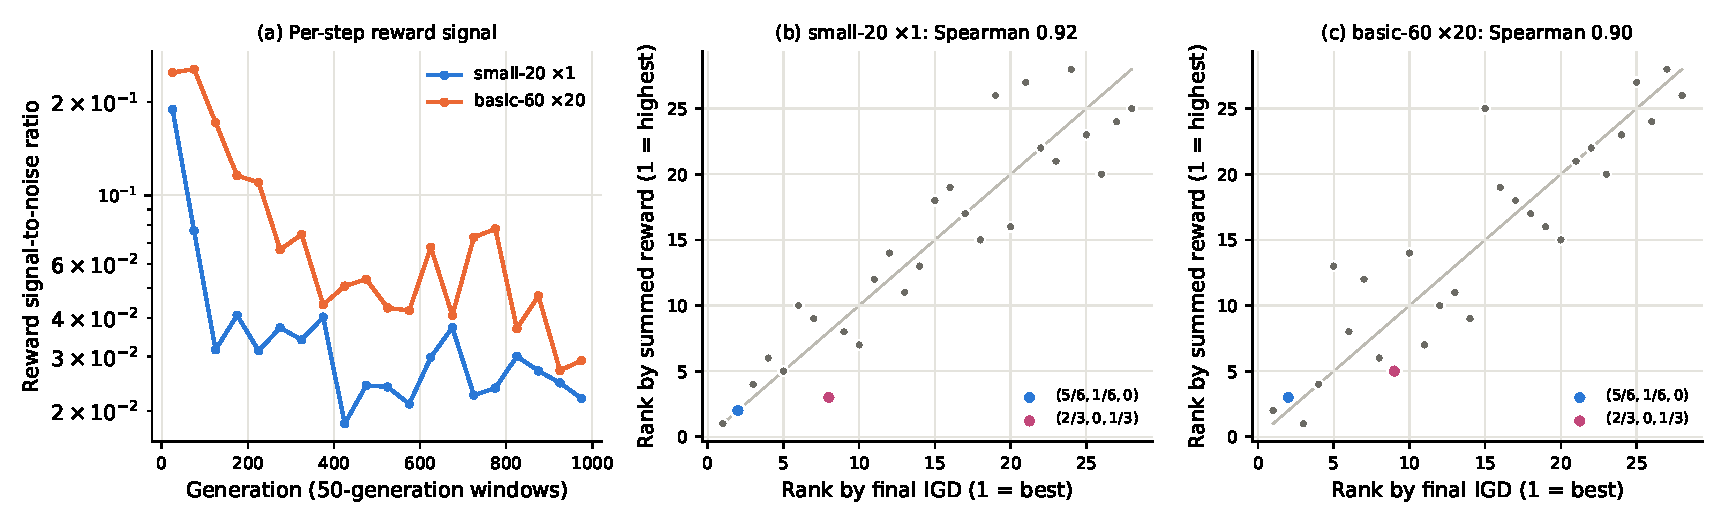
\includegraphics[width=\textwidth]{figures/d1_reward_audit.pdf}
\caption{Reward audit, each of the 28 actions held fixed for 1000 generations. (a) Signal-to-noise ratio of the
per-generation reward. (b, c) Rank of the summed reward against rank by final IGD.}
\label{fig:reward_audit}
\end{figure*}
    % 5   ~5 pages
% Discussion and limitations: placeholder until step 5 condenses sections/validity.tex into this file.
% Threats to validity and limitations (R3). Every number is from the generated tables in paper/tables
% (scripts/build_paper.py) or from PLAN.md entries B1, B4, E2, E6, E7, A1b and the scalability study.
\section{Threats to validity and limitations}
\label{sec:validity}

\paragraph{Metrics and normalisation (construct validity)}
IGD and HV are computed after normalising each instance once, over the final fronts of all compared methods, and
IGD is measured against the non-dominated union of those fronts. The verdict between two strong methods can depend
on which methods form that pool. Table~\ref{tab:robustness} repeats the comparison of \ours{} with IMOEA/D under four
pools. On Suite A and on the Suite B workflows with up to 400 tasks, every pool gives the same verdict. On HV the
Suite B record is also stable (42 wins, 2 losses, 1 tie in three of the four pools, 42/1/2 in the fourth). On IGD
at 1000 tasks it is not: with the pool of the main tables \ours{} is better on 14 of the 15 instances, but when the
weak baselines are left out of the pool IMOEA/D has the lower IGD on 6--9 of them. We therefore report HV as the
headline metric at 1000 tasks and state that IGD there is level or favours IMOEA/D. The Monte Carlo shares of
Table~\ref{tab:montecarlo} are subject to the same caveat, because each scenario's crisp reference front is pooled
over the same methods. Imprecision is the sum of the interval widths over the final front, so methods whose fronts
collapse to a few solutions, such as IMOEA-DQN, score best on it; it has to be read together with IGD and HV.

\paragraph{Uncertainty model}
The model assumes that every uncertain quantity stays inside its interval. The Monte Carlo check
(Table~\ref{tab:montecarlo}) confirms that the predicted objective intervals contain the realised values in all of
200 scenarios per instance, but those scenarios draw every input uniformly and independently; correlated
fluctuations (for example a shared channel degrading for all devices at once) and values outside the stated bounds
were not tested. The interval half-widths of task workloads and data sizes in Suite B are synthetic (5--30\% of the
midpoint, drawn per task), and Suite A tasks are crisp, as in Jin et al., so that uncertainty there comes only from
the resources. A sensitivity run with half and double the half-widths (Table~\ref{tab:sensitivity}) keeps \ours{}
ahead on IGD, but with doubled widths IMOEA/D wins HV on 2 of 5 workflows.

\paragraph{System model simplifications (external validity)}
The evaluator makes the following simplifications. Concurrent transfers do not share bandwidth, so there is no link
contention. An edge server divides its capacity equally and statically among all tasks placed on it instead of
scheduling them over time; a variant in which edge servers queue tasks gives the same ranking
(Table~\ref{tab:sensitivity}). The cloud runs every task in parallel. The device spends energy on local computation,
on transmission and while idle, but not on receiving data. Following Jin et al., the main setting counts only the
device's energy and uses a fixed channel gain. When the energy of all three tiers is counted instead, the comparison
with IMOEA/D becomes close (IMOEA/D better on IGD in 3 of 5 workflows and on HV in 4 of 5,
Table~\ref{tab:sensitivity}). Finally, the problem is static and offline: every application is known before the
optimisation starts, and no tasks arrive during execution. All results are from simulation; we have not run the
schedules on a testbed.

\paragraph{Benchmarks}
Suite A follows Jin et al.'s instance sizes with randomly generated layered DAGs; Suite B uses five WfCommons
workflow families whose workloads and data sizes were mapped into Jin et al.'s ranges by an order-preserving
logarithmic map. The instances cover 3--10 edge servers and up to 2000 tasks. Other application structures, larger
edge deployments or real traces may behave differently.

\paragraph{Baselines (internal validity)}
All baselines were re-implemented on the same encoding, operators, evaluator, population size and number of
evaluations as \ours{}, from the descriptions in their papers rather than the authors' code. Where a paper leaves a detail open
we chose the most literal reading and documented it. The original IP-MOEA paper was not obtainable; its crowding is
implemented as the hypervolume contribution described by later papers that use it as a baseline, which is both closer
to that description and stronger than a midpoint crowding distance. IMOEA/D uses the original settings reported in
the IMEA-IED paper ($T = 10$, weight adaptation from $G_{\max}/2$ every $G_{\max}/6$). IMOEA/D-AWN evaluates
$NG_{\max}$ solutions instead of $N(G_{\max} + 1)$, as published (0.1\% fewer). IMaOEACI was left out because its
central indicator is defined only in an unpublished thesis. For IMOEA-DQN, the experience-replay threshold and the
exploration schedule are not given in the paper (we use 250 transitions and $\varepsilon_t = 0.3^{t/100}$), and its
simulated binary crossover cannot keep a task order topological, so it uses our operators. Baselines run with their
published parameters, not retuned for this problem.

\paragraph{Tuning and statistics (conclusion validity)}
The selection weights $(5/6, 1/6, 0)$ and the mating parameters $T = 10$, $p_{local} = 1.0$ were chosen on separate
training instances of Suite A (instances i1--i3) and frozen before any test run; the test instances (i0 and Suite B)
were never used for tuning. \ours{}, IMOEA/D and the Jin backbone were run 30 times per instance and every other
method 10 times. The Wilcoxon tests are Holm-corrected over the methods compared on one instance, not across the 57
instances; across instances we rely on the Friedman test, whose Nemenyi critical difference is large on Suite A's 12
instances (3.91 ranks). Wall-clock times come from one laptop; re-timing \ours{} with the same settings in a later batch gave times 0.82--1.21
times the first ones, so differences below about 20\% are not meaningful.

\paragraph{Remaining weaknesses of the method}
Two results do not favour \ours{}. First, on the 100-task Suite B workflows with the smallest data sizes, NSGA-II
reaches a lower IGD on 4--5 of 45 instances (Table~\ref{tab:suiteb_igd}), probably because the search space is small
enough for plain non-dominated sorting to converge. Second, at 1000--2000 tasks IMOEA/D reaches cheaper solutions
at the cost end of the front. Where the two fronts overlap, \ours{}'s dominates 61--90\% of IMOEA/D's and almost none
the other way, and \ours{} keeps the higher HV on 13 of the 15 2000-task instances (Table~\ref{tab:scalability}). Yet
IMOEA/D's better coverage of the cost extreme decides IGD at that size: there, IMOEA/D is better on 5, worse on 6
and tied on 4 instances. Neither a doubled budget ($G_{\max} = 2000$), nor a running normalisation of the Tchebycheff
rank, nor extra weight vectors near the axes closed this gap in a pilot study; it appears to come from IMOEA/D's
steady-state replacement per subproblem.

\paragraph{Scope of the negative result on learned control}
The finding that learned control of $(\alpha, \beta, \gamma)$ does not beat the best fixed action
(Tables~\ref{tab:learners} and \ref{tab:gat}) holds for the three learner designs we tried: per-generation, per-block
and restricted-action DQN, with and without a graph-attention state encoder, trained for 24--48 episodes on the
Suite A training instances. A different state representation, reward or much larger training budget might change it.
The reward audit (Fig.~\ref{fig:reward_audit}) explains the difficulty: once the population has converged, the
per-generation reward carries a signal-to-noise ratio of 0.02--0.08, and the best fixed action is already within
about 10\% of the best per-instance action, which leaves little room for an adaptive schedule to gain.

     % 6   ~0.75 page
% Conclusion (draft).
\section{Conclusion}
\label{sec:conclusion}

We formulated the offloading of DAG workflows in cloud--edge--end systems with interval-valued resources and workloads
as an interval multi-objective problem over task placement and task order, with makespan computed along the interval
critical path, device energy and cost as objectives. Extending the three-tier selection of IMOEA-DQN to this problem
showed that its convergence ranking, the interval dominance degree, stops selecting once most of the population is
mutually non-dominated, and that its learned control of the selection weights does not beat a fixed choice. \ours{}
replaces the convergence ranking with an interval version of the MSOPS best-position Tchebycheff rank, breaks its ties
by crowding distance, mates neighbours in objective space and fixes the selection weights on training instances.

On Jin et al.'s instance sizes \ours{} has the best IGD and hypervolume on every instance, and on five families of
scientific workflows with 100 to 1000 tasks it is better than the strongest baseline, IMOEA/D, on 43 of 45 instances in
IGD and 42 in hypervolume, at about the same running time. The ablation attributes the gain to the new rank and the
neighbourhood mating together, and the predicted objective intervals contain every realised value in a Monte Carlo
check. At 1000 and 2000 tasks the advantage narrows: \ours{} keeps the higher hypervolume, but IMOEA/D reaches cheaper
solutions at the cost end of the front and IGD becomes level and dependent on the reference front.

Three directions follow. The first is to close the gap at the cost extreme on large workflows, for example by
combining the three-tier selection with steady-state replacement per subproblem, which our analysis points to as the
source of IMOEA/D's advantage there. The second is to make the model more realistic: shared link bandwidth, receive
energy, time-varying edge capacity, correlated uncertainty and applications that arrive online. The third is a small
uncertainty share in the selection weights, which narrowed the intervals by 10\% at a small cost in IGD on the training
instances and may suit settings where predictable performance matters more than the best expected value.
     % 7   ~0.4 page

% ---------------------------------------------------------------- floats in the main text (4 figures, 4 tables)
\begin{figure*}[!t]
\centering
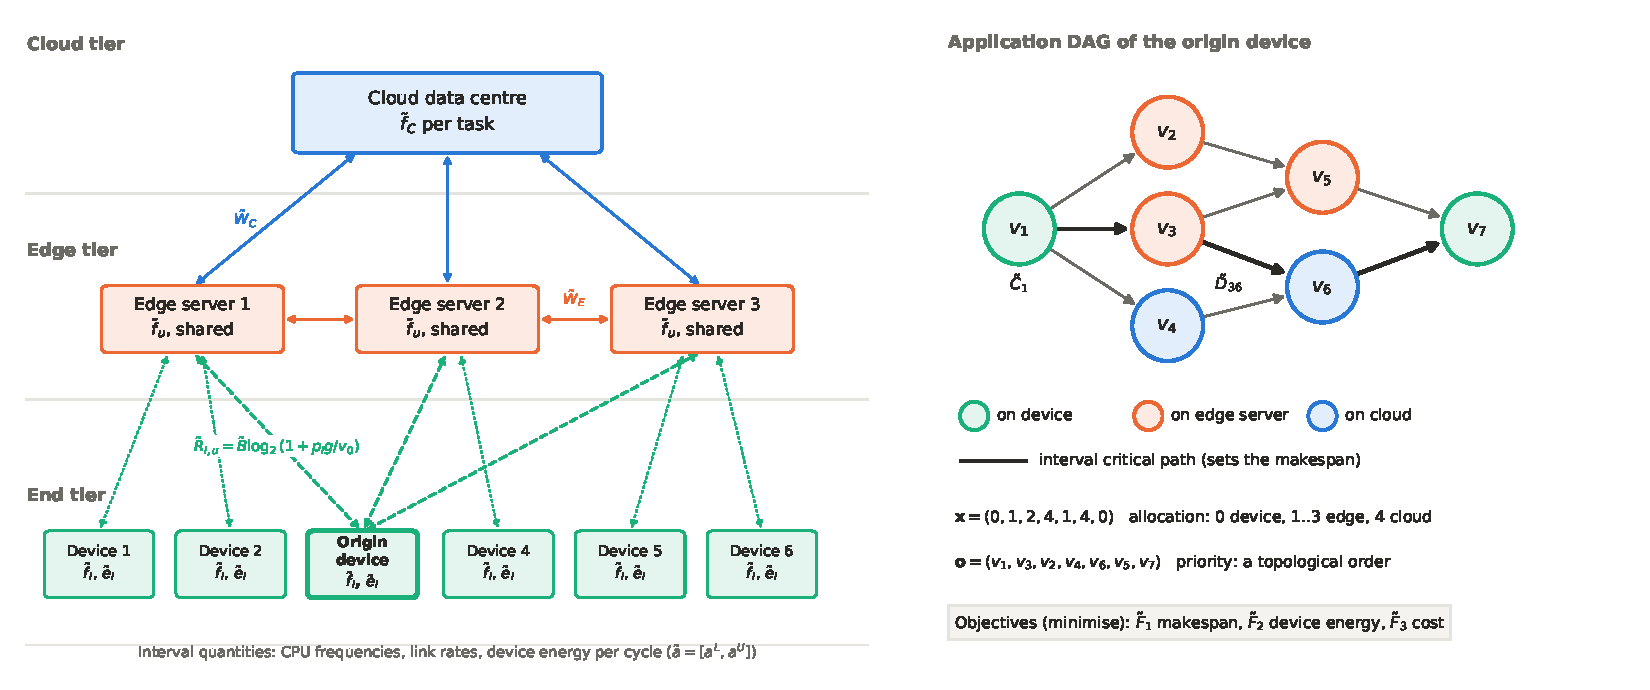
\includegraphics[width=0.9\textwidth]{figures/system_model.pdf}
\caption{System model. Left: the cloud--edge--end architecture with its interval quantities. Right: an application
DAG submitted by the origin device, with its tasks coloured by the tier the allocation string assigns them to, a
priority string, and the interval critical path that determines the makespan.}
\label{fig:system_model}
\end{figure*}

% generated by scripts/build_paper.py; do not edit by hand
\begin{table*}[!htbp]
\centering
\footnotesize
\caption{Results on both suites: mean IGD ($\times10^{-2}$) and HV over instances, the number of instances on which each method is significantly better / worse / not different from \ours{} (Wilcoxon rank-sum, Holm-corrected, $\alpha = 0.05$), and the mean Friedman rank by IGD (Nemenyi critical difference 3.91 on Suite A, 2.02 on Suite B). Per-instance results are in the supplementary material.}
\label{tab:summary}
\setlength{\tabcolsep}{3pt}
\begin{tabular}{lcccccccccc}
\toprule
& \multicolumn{5}{c}{Suite A (12 instances)} & \multicolumn{5}{c}{Suite B (45 instances)} \\
\cmidrule(lr){2-6}\cmidrule(lr){7-11}
Method & IGD & HV & IGD $+/-/\approx$ & HV $+/-/\approx$ & Rank & IGD & HV & IGD $+/-/\approx$ & HV $+/-/\approx$ & Rank \\
\midrule
\ours{} & \textbf{1.22} & \textbf{0.819} & -- & -- & 1.00 & \textbf{1.86} & \textbf{0.949} & -- & -- & 1.29 \\
IMOEA/D & 3.19 & 0.797 & 0/12/0 & 0/12/0 & 2.83 & 2.57 & 0.935 & 1/43/1 & 2/42/1 & 2.69 \\
IMOEA/D-AWN & 2.91 & 0.797 & 0/12/0 & 0/12/0 & 2.42 & 4.44 & 0.915 & 0/43/2 & 0/44/1 & 3.29 \\
IMEA-IED & 12.40 & 0.691 & 0/12/0 & 0/12/0 & 7.17 & 13.34 & 0.828 & 0/45/0 & 0/45/0 & 7.73 \\
IP-MOEA & 14.71 & 0.658 & 0/12/0 & 0/12/0 & 8.50 & 12.24 & 0.822 & 0/45/0 & 0/45/0 & 6.98 \\
NSGA-II (mid) & 4.84 & 0.770 & 0/12/0 & 0/12/0 & 4.50 & 6.51 & 0.882 & 4/40/1 & 0/44/1 & 3.82 \\
NSGA-II (int) & 4.80 & 0.771 & 0/12/0 & 0/12/0 & 4.25 & 6.57 & 0.882 & 5/40/0 & 0/44/1 & 4.09 \\
NSGA-III & 13.61 & 0.690 & 0/12/0 & 0/12/0 & 7.75 & 15.42 & 0.822 & 0/45/0 & 0/45/0 & 8.40 \\
Jin backbone & 11.66 & 0.635 & 0/12/0 & 0/12/0 & 6.67 & 11.64 & 0.805 & 0/45/0 & 0/45/0 & 6.78 \\
IMOEA-DQN & 25.43 & 0.605 & 0/12/0 & 0/12/0 & 9.92 & 22.94 & 0.736 & 0/45/0 & 0/45/0 & 9.93 \\
\bottomrule
\end{tabular}
\end{table*}


\begin{figure*}[!t]
\centering
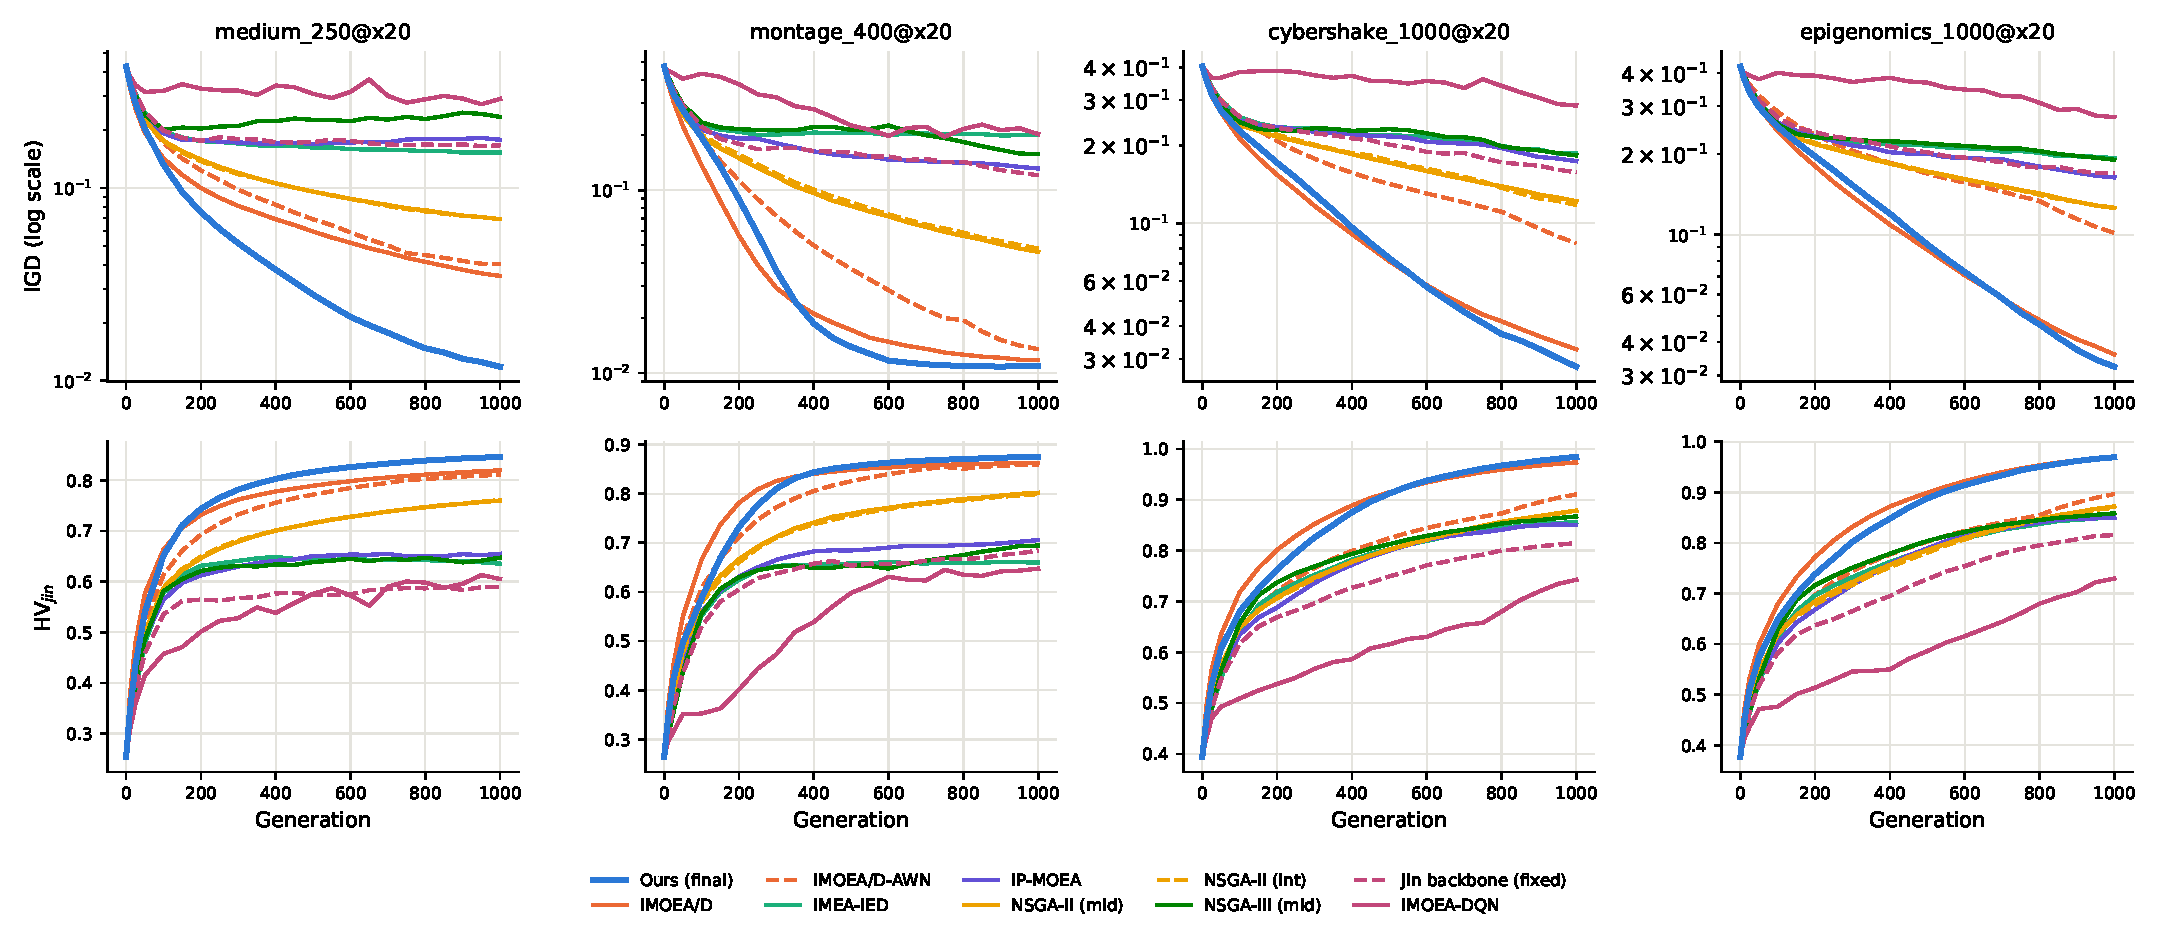
\includegraphics[width=\textwidth]{figures/e5_convergence.pdf}
\caption{Mean IGD (top, log scale) and HV (bottom) against the generation, 10 runs per method.}
\label{fig:e5_convergence}
\end{figure*}

% generated by scripts/build_paper.py; do not edit by hand
\begin{table}[!htbp]
\centering
\footnotesize
\caption{Ablation on the 12 Suite A instances (10 runs; IGD $\times10^{-2}$, means over instances). $+/-/\approx$: instances where the variant is significantly better / worse / not different from the reference in the group heading (Wilcoxon rank-sum, $\alpha = 0.05$).}
\label{tab:ablation}
\setlength{\tabcolsep}{3pt}
\begin{tabular}{lccc}
\toprule
Variant & IGD & HV & IGD $+/-/\approx$ \\
\midrule
\multicolumn{4}{l}{\textit{Build-up (vs \ours{})}} \\
\quad Jin et al.\ backbone & 11.86 & 0.630 & 0/12/0 \\
\quad + Tchebycheff Rank C & 5.76 & 0.760 & 0/12/0 \\
\quad + ICD tie-break & 4.80 & 0.769 & 0/12/0 \\
\quad + mating, $T{=}20$, $p{=}0.9$ & 1.35 & 0.806 & 0/9/3 \\
\quad \ours{} ($T{=}10$, $p{=}1$) & 1.02 & 0.814 & -- \\
\midrule
\multicolumn{4}{l}{\textit{Leave one out (vs $T{=}20$)}} \\
\quad without Tchebycheff & 6.83 & 0.664 & 0/12/0 \\
\quad without ICD tie-break & 1.63 & 0.801 & 0/8/4 \\
\quad without mating & 4.80 & 0.769 & 0/12/0 \\
\midrule
\multicolumn{4}{l}{\textit{Parameters (vs $T{=}20$)}} \\
\quad $T = 10$ & 1.07 & 0.812 & 9/0/3 \\
\quad $T = 40$ & 2.38 & 0.792 & 0/12/0 \\
\quad $p_{local} = 0.5$ & 2.01 & 0.796 & 0/11/1 \\
\quad $N/2$ weight vectors & 1.80 & 0.803 & 0/12/0 \\
\quad $2N$ weight vectors & 1.90 & 0.792 & 0/11/1 \\
\quad action $(1, 0, 0)$ & 1.75 & 0.801 & 0/7/5 \\
\bottomrule
\end{tabular}
\end{table}

% generated by scripts/build_paper.py; do not edit by hand
\begin{table}[!htbp]
\centering
\footnotesize
\caption{Sensitivity on the five 400-task workflows (data $\times 20$, 10 runs), one setting changed at a time, and scalability to 2000 tasks. Last two columns: instances where IMOEA/D is significantly better / worse / not different from \ours{} (Wilcoxon rank-sum, Holm, $\alpha = 0.05$). NSGA-II and the Jin backbone are worse on every instance in every setting (Table~\Sref{tab:sensitivity} of the supplementary material).}
\label{tab:sensitivity}
\setlength{\tabcolsep}{3pt}
\begin{tabular}{lcccc}
\toprule
& \multicolumn{2}{c}{IGD ($\times10^{-2}$)} & \multicolumn{2}{c}{IMOEA/D $+/-/\approx$} \\
\cmidrule(lr){2-3}\cmidrule(lr){4-5}
Setting & Ours & IMOEA/D & IGD & HV \\
\midrule
Base case & \textbf{0.82} & 1.21 & 0/5/0 & 0/5/0 \\
All-tier energy & \textbf{1.00} & 1.08 & 3/1/1 & 4/0/1 \\
Widths $\times 0.5$ & \textbf{0.94} & 1.78 & 0/5/0 & 0/5/0 \\
Widths $\times 2$ & \textbf{0.73} & 0.89 & 0/4/1 & 2/1/2 \\
Bandwidth $\times 0.5$ & \textbf{1.18} & 1.60 & 0/5/0 & 0/5/0 \\
Bandwidth $\times 2$ & \textbf{0.63} & 1.00 & 0/5/0 & 0/5/0 \\
1 edge server & \textbf{0.93} & 1.12 & 0/4/1 & 0/4/1 \\
6 edge servers & \textbf{1.08} & 1.70 & 0/4/1 & 0/5/0 \\
Edge queueing & \textbf{0.83} & 1.06 & 0/5/0 & 0/4/1 \\
\midrule
2000 tasks & 6.99 & \textbf{6.92} & 5/6/4 & 0/13/2 \\
\bottomrule
\end{tabular}
\end{table}

% generated by scripts/build_paper.py; do not edit by hand
\begin{table}[!htbp]
\centering
\footnotesize
\caption{Learned against fixed control of the selection weights on four Suite A instances (4 runs; IGD $\times10^{-2}$). All rows above \ours{} use the Tchebycheff backbone with $T = 20$, $p_{local} = 0.9$. $+/-/\approx$: instances where the row is significantly better / worse / not different from the fixed action $(5/6, 1/6, 0)$ (Wilcoxon rank-sum, $\alpha = 0.05$).}
\label{tab:learners}
\setlength{\tabcolsep}{3pt}
\begin{tabular}{lccc}
\toprule
Control of $(\alpha, \beta, \gamma)$ & IGD & HV & IGD $+/-/\approx$ \\
\midrule
\multicolumn{4}{l}{\textit{Fixed or random action}} \\
\quad Fixed $(5/6, 1/6, 0)$ & 1.43 & 0.784 & -- \\
\quad Fixed $(1, 0, 0)$ & 1.77 & 0.778 & 0/1/3 \\
\quad Random, $\alpha \ge 1/2$ & 2.51 & 0.751 & 0/4/0 \\
\midrule
\multicolumn{4}{l}{\textit{DQN control (interval, reward, actions)}} \\
\quad Every gen., PIBI, GAT & 3.67 & 0.759 & 0/4/0 \\
\quad Every gen., PIBI & 3.22 & 0.760 & 0/4/0 \\
\quad Every 50 gen., HV, GAT & 7.31 & 0.720 & 0/4/0 \\
\quad Every 50 gen., HV & 5.41 & 0.739 & 0/4/0 \\
\quad Every 25 gen., 10 act., GAT & 2.23 & 0.774 & 0/3/1 \\
\quad Every 25 gen., 10 act. & 1.96 & 0.778 & 0/2/2 \\
\midrule
\multicolumn{4}{l}{\textit{For comparison}} \\
\quad \ours{} & 1.21 & 0.792 & 3/0/1 \\
\quad IMOEA-DQN & 23.88 & 0.583 & 0/4/0 \\
\quad IMOEA/D & 2.92 & 0.770 & 0/4/0 \\
\bottomrule
\end{tabular}
\end{table}


\begin{figure*}[!t]
\centering
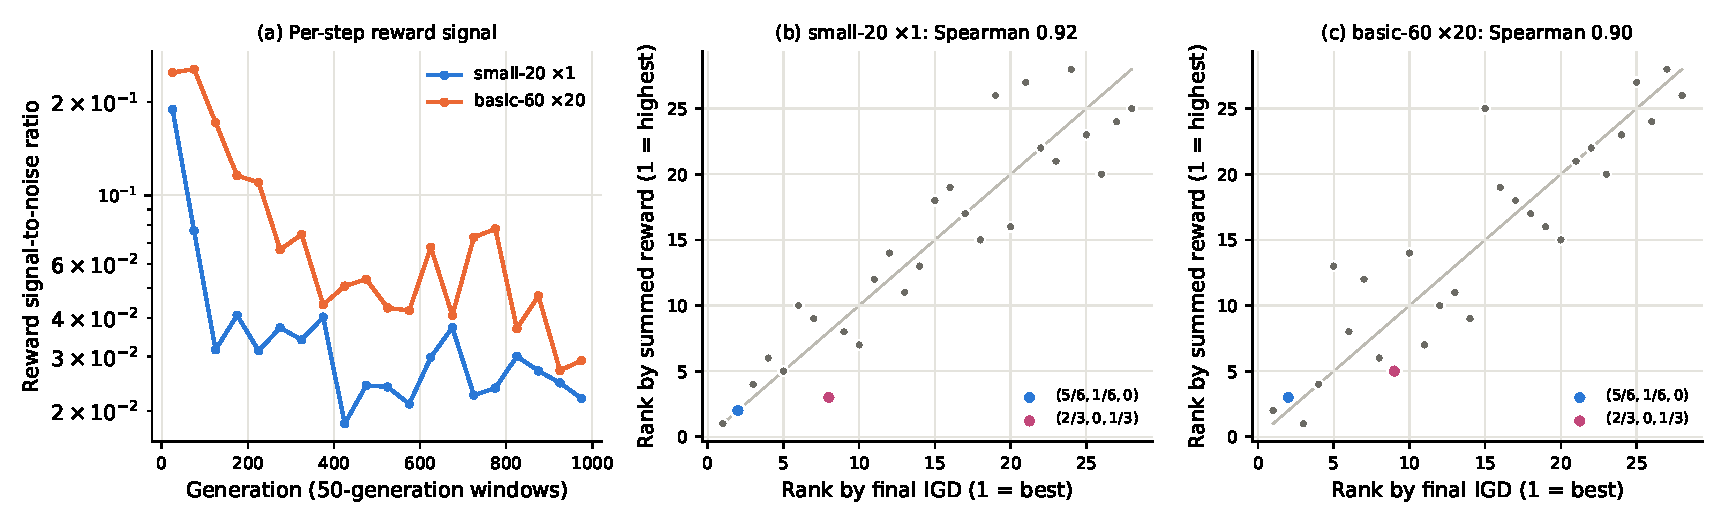
\includegraphics[width=\textwidth]{figures/d1_reward_audit.pdf}
\caption{Reward audit, each of the 28 actions held fixed for 1000 generations. (a) Signal-to-noise ratio of the
per-generation reward. (b, c) Rank of the summed reward against rank by final IGD.}
\label{fig:reward_audit}
\end{figure*}

% ---------------------------------------------------------------- back matter
\printcredits

\section*{Declaration of competing interest}
\todo{competing-interest statement}

\section*{Data availability}
\todo{state where the code, instances and results are available}

\bibliographystyle{cas-model2-names}
\bibliography{refs}

\end{document}
